The efficiency corresponding to the \egamma\ part of the photon ID is estimated by exploiting \PZ\ boson decays into pairs of electrons and positrons.
Using the TP method, a high-quality electron object (tag) is identified in a single photon data sample, and the accompanying electron is sought for in the pool of elecromagnetic objects (probes) in the event. 
The area under the peak in the mass distribution of the tag-probe system around the \PZ\ boson mass (between 81\GeV\ and 101\GeV) is then measured once applying the \Pe\Pgg\ ID requirements on the probe and once inverting all of the requirements simultaneously. 
Denoting the two areas under the peaks in the passing and failing samples \npass\ and \nfail, respectively, the resulting effiency $\epsilon_{\egamma}$ is given by
\begin{equation}
\epsilon_{\egamma} = \frac{\npass}{\npass + \nfail}.
\end{equation}

The TP measurement is performed on a subset of the single photon triggered events where there is an electron object (tag) passing the ``tight'' identification criteria in addition to the triggering photon (probe). 
All possible tag-probe combinations are considered; if the tag object can also serve as a probe and the probe object as a tag, which is a common occurrence in the case when the probe is electron-like (passes the \Pe\Pgg\ ID), then the two combinations are considered independently to avoid the bias caused by preferring to use one object over another as the probe.

The tag-probe mass distributions are then fit to extract \npass\ and \nfail. 
The fit model is composed of two templates, where one template describes a pure \Zee\ line shape and the other describes the background contributions. 
The backgrounds to the fits include \wj, diboson, and \ttbar\ productions, which are all negligible and estimated to contribute by less than 1\%. 
Minor contributions from processes that do not involve true electrons, such as diphoton production with a strongly asymmetric conversion on one of the photons and misidentification of a QCD jet as an electron, are predicted to be negligible from MC studies.
 
The \Zee\ template shape is an analytic convolution of the Breit-Wigner distribution and the Crystal Ball function. 
The mass and width parameters of the Breit-Wigner distribution are fixed to PDG values while the Crystal Ball parameters are allowed to float in the fit.
We are able to use the analytic Breit-Wigner distribution instead of a template taken from MC because at this high probe \pt\ scale the selected events are mostly of the \zj\ topology with a boosted \PZ\ boson.
This makes the selection rather inclusive in terms of the tag-probe invariant mass and ensures that the Breit-Wigner distribution accurately models the mass distribution even through the tag and probe are under kinematically exclusive selections.

\begin{figure}[htbp]
  \centering
  \resizebox{0.95\textwidth}{!}{
    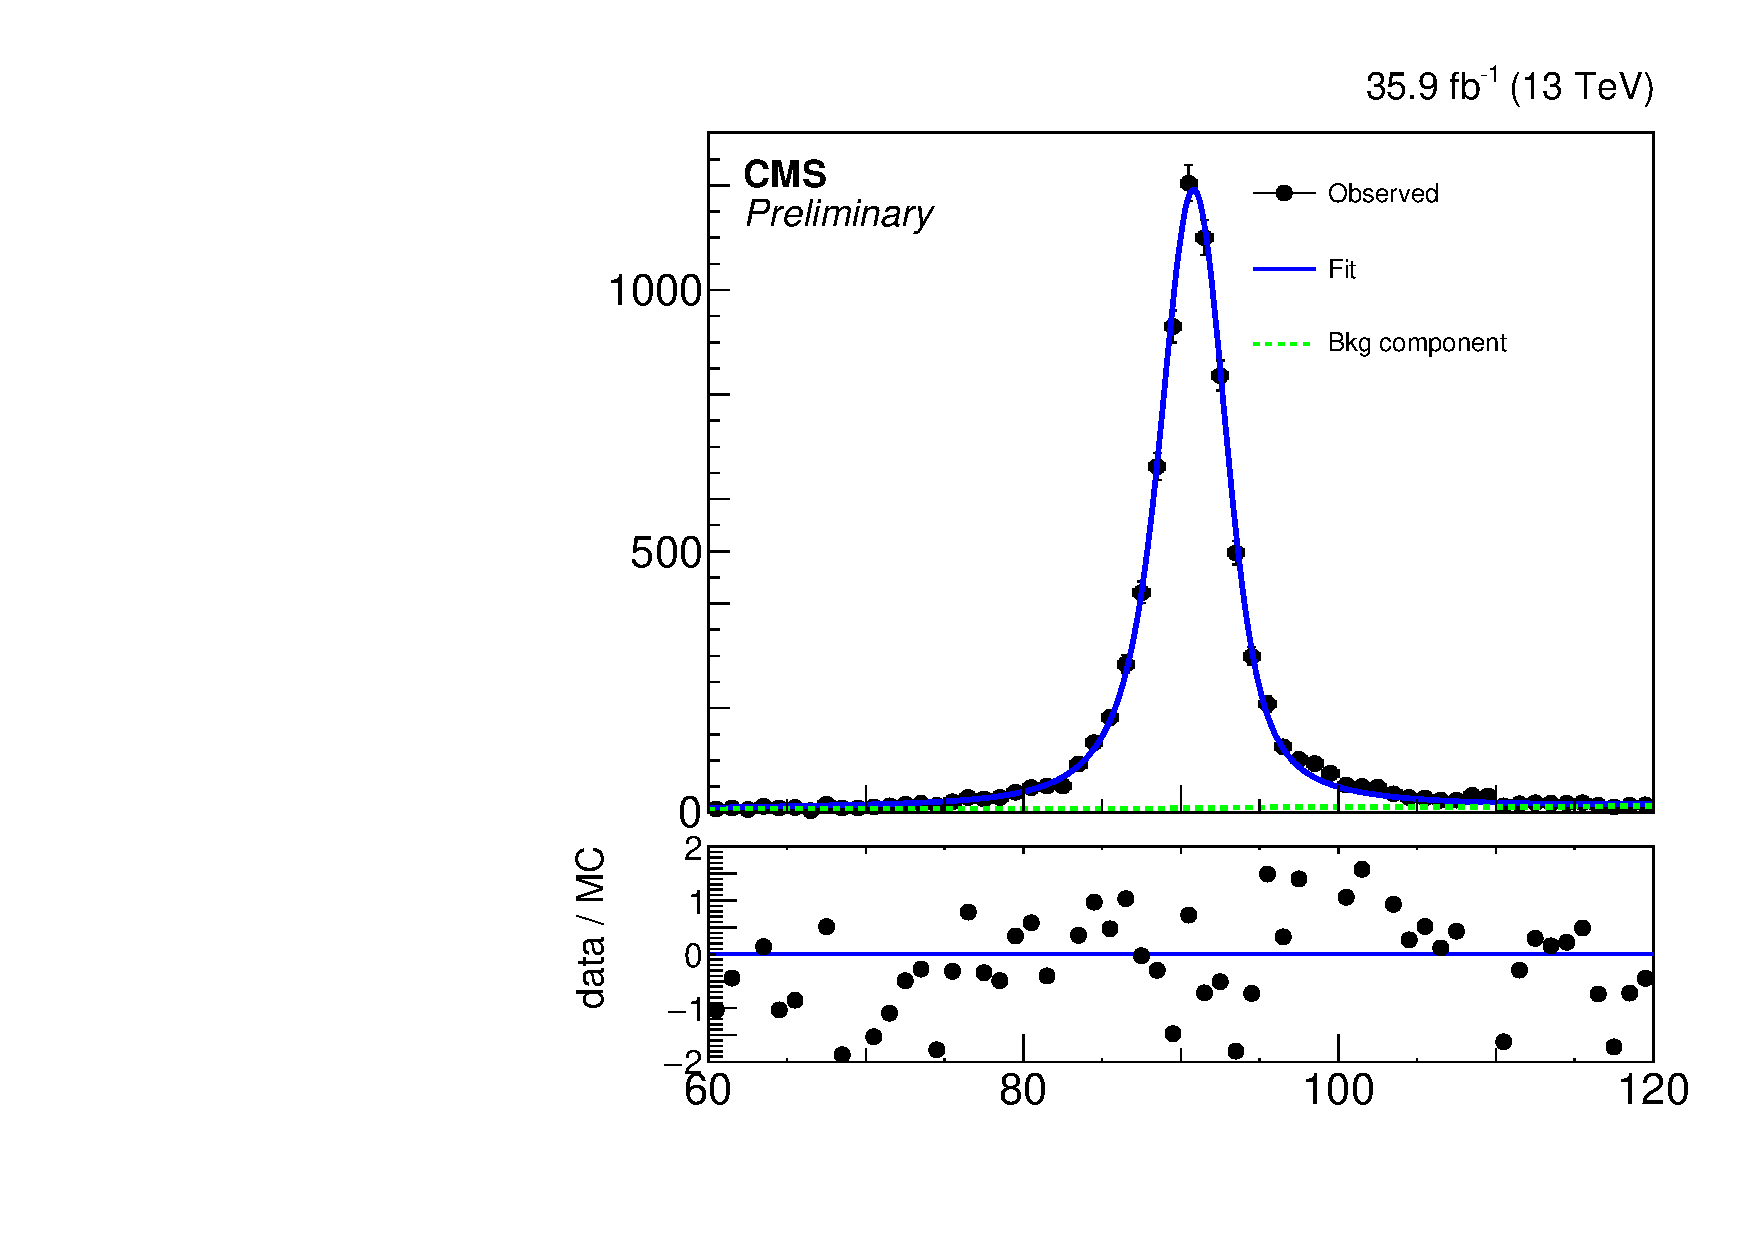
\includegraphics[]{Calibration/Figures/idsf/fit_data_pass_pt_175_200.pdf}
    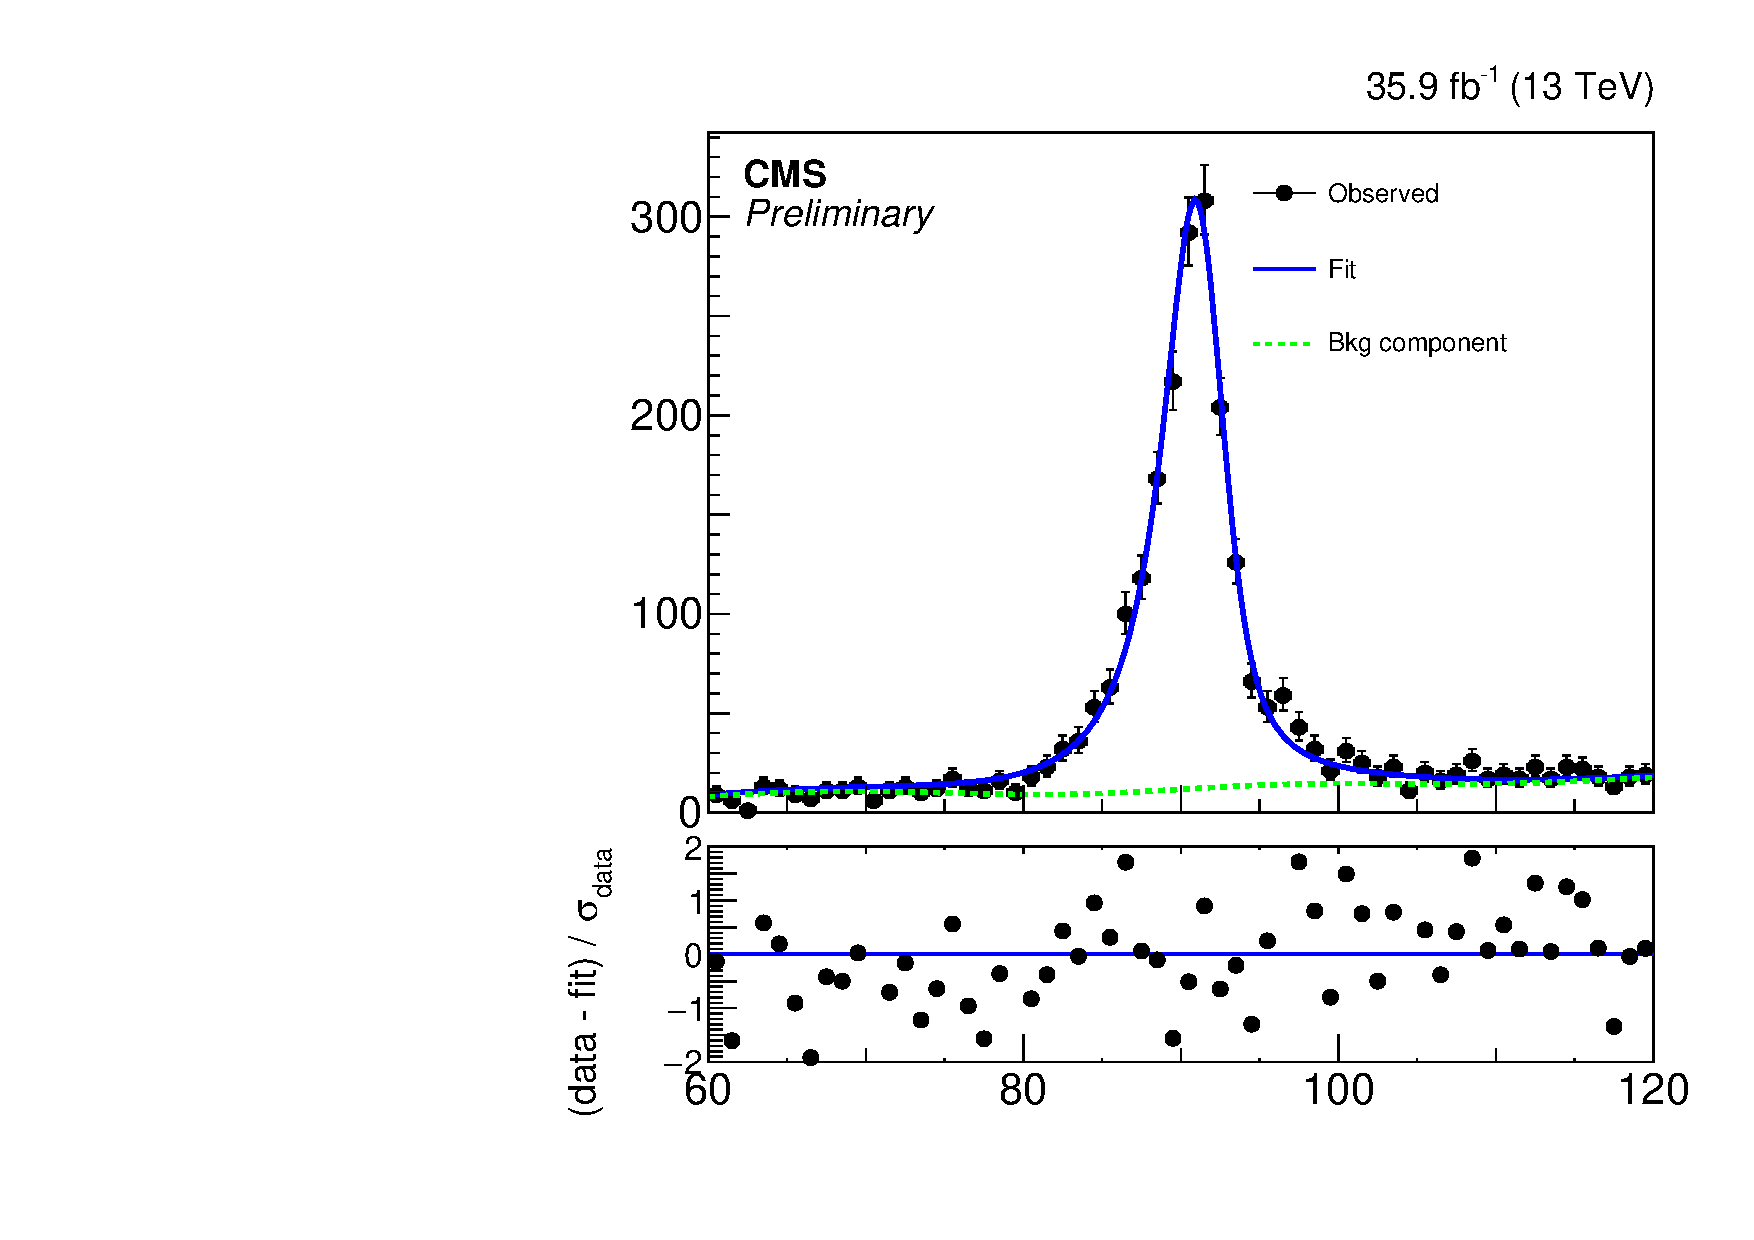
\includegraphics[]{Calibration/Figures/idsf/fit_data_fail_pt_175_200.pdf}
  }
  \resizebox{0.95\textwidth}{!}{
    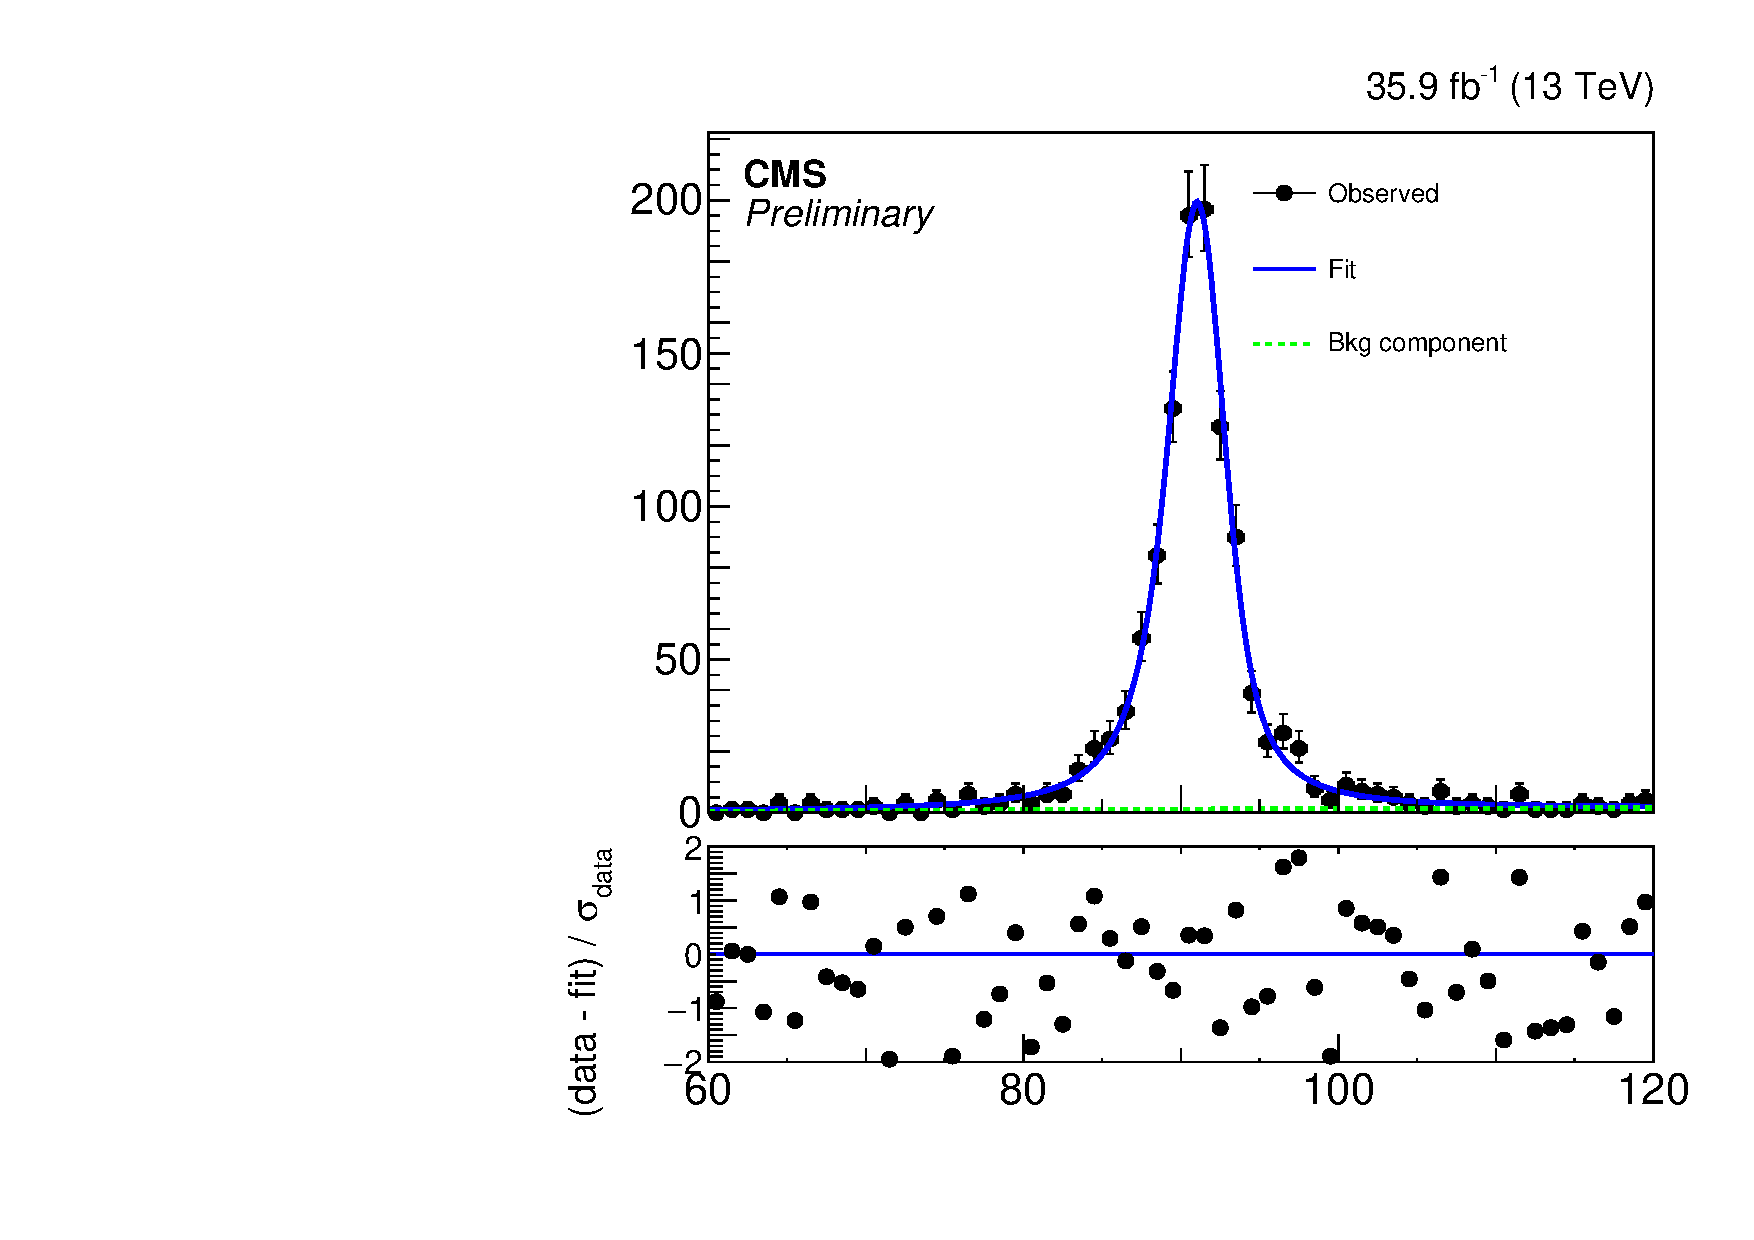
\includegraphics[]{Calibration/Figures/idsf/fit_data_pass_pt_300_350.pdf}
    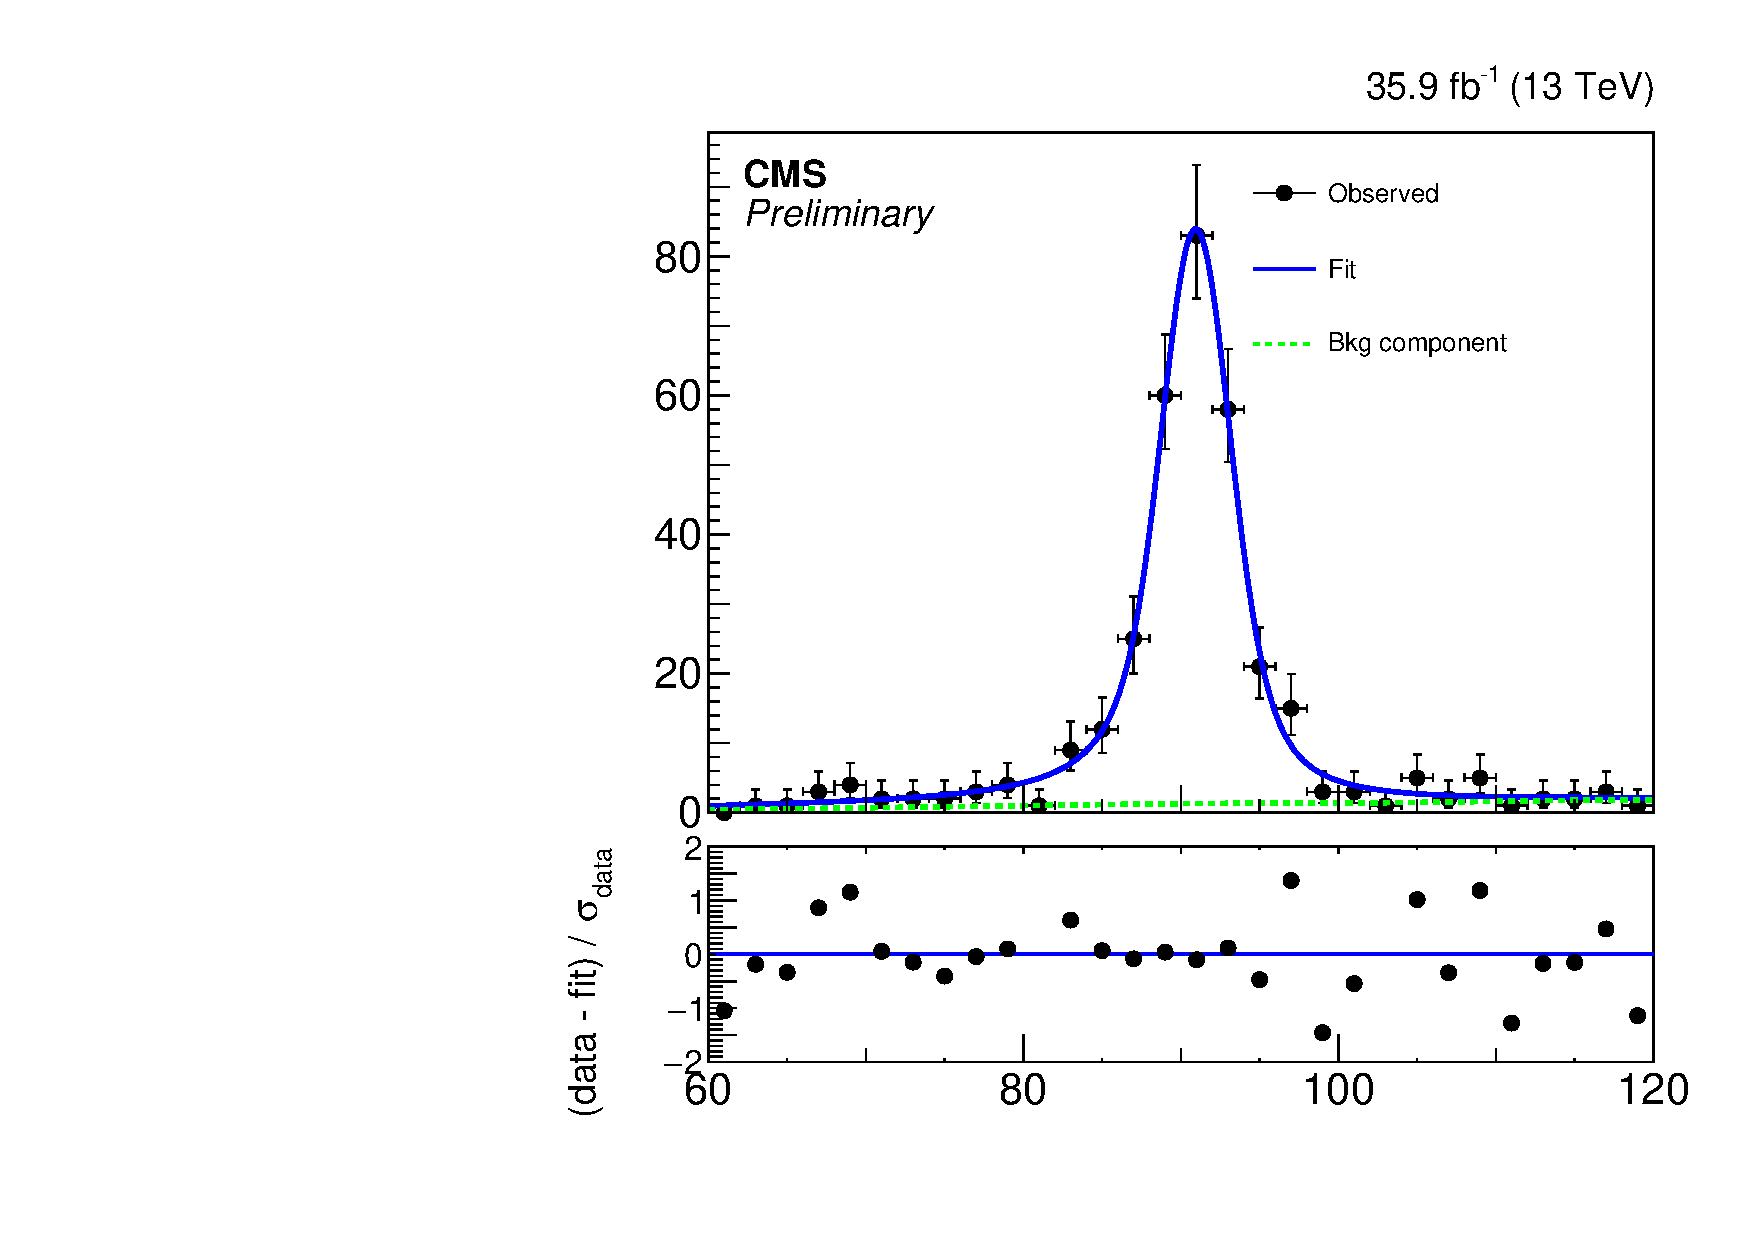
\includegraphics[]{Calibration/Figures/idsf/fit_data_fail_pt_300_350.pdf}
  }
  \resizebox{0.95\textwidth}{!}{
    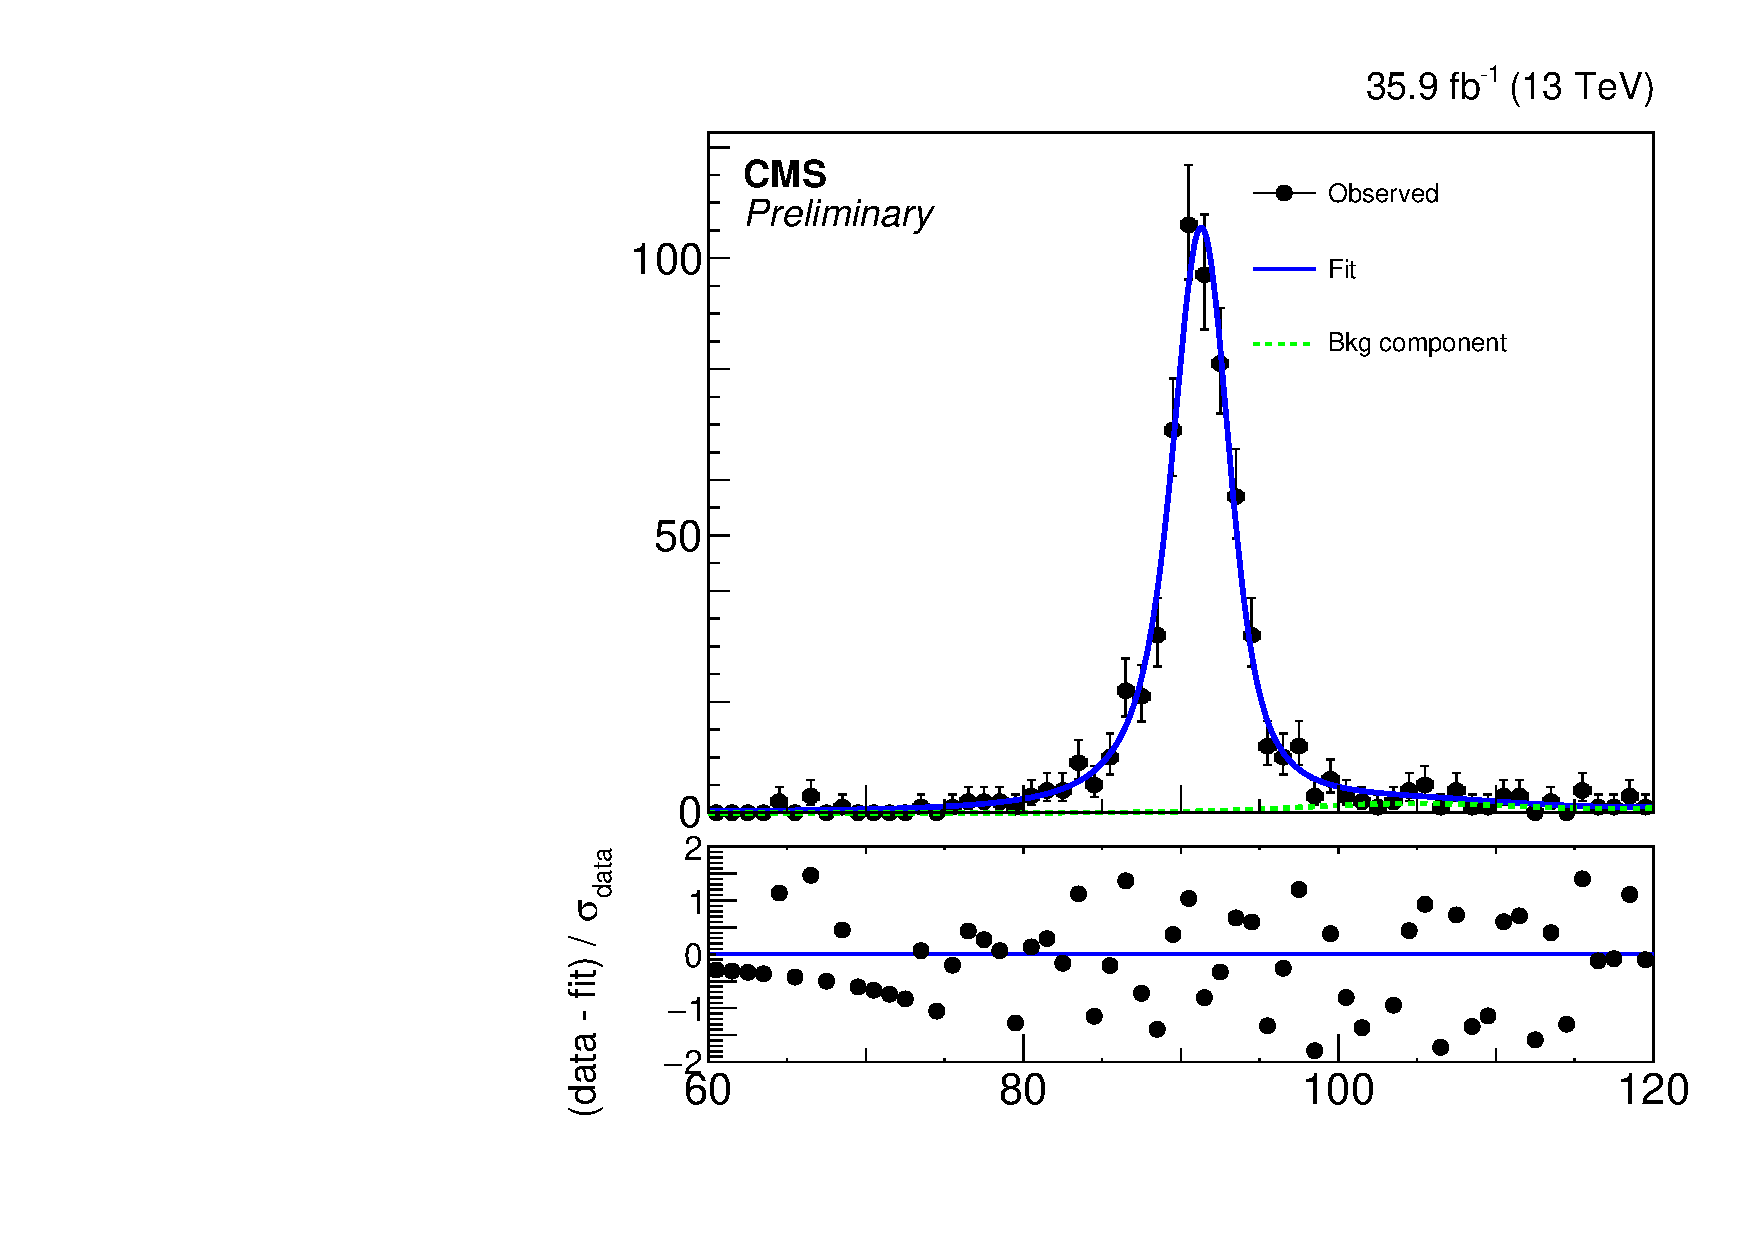
\includegraphics[]{Calibration/Figures/idsf/fit_data_pass_pt_400_6500.pdf}
    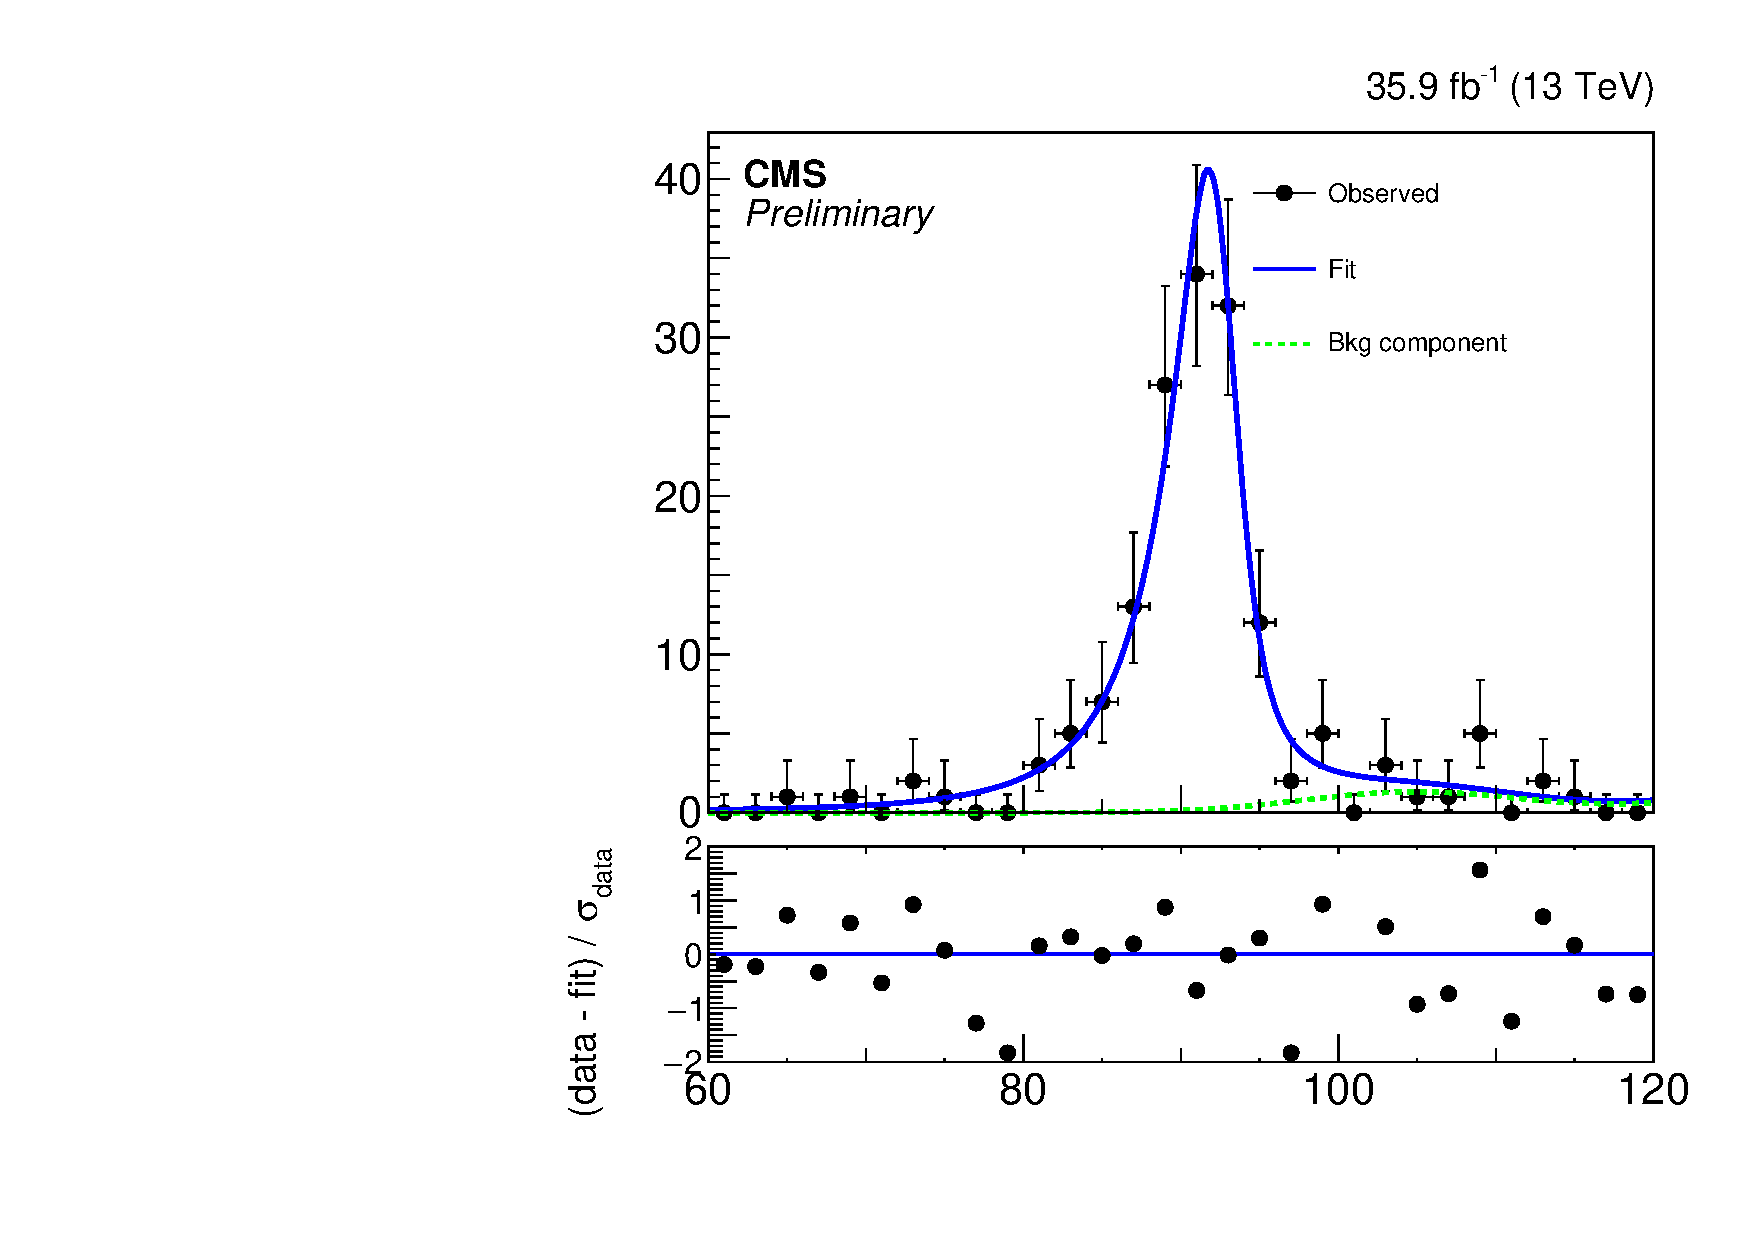
\includegraphics[]{Calibration/Figures/idsf/fit_data_fail_pt_400_6500.pdf}
  }
  \caption{
    Fits to the mass distributions for pass (left) and fail (right) selections, in bins of probe \pt: 
    $175 < \pt < 200\GeV$ (top), 
    $300 < \pt < 350\GeV$ (middle), 
    $\pt > 400\GeV$ (bottom). 
    The blue solid line represents the full fit model, and the green dashed line its background component.
  }
  \label{fig:idsf_fits}
\end{figure}

The background template is taken from events collected by the single photon trigger where an additional muon object is present, making use of the fact that the most of the background processes in both fits are symmetric in lepton flavor. 
In order to mitigate statistical fluctuations in the background sample, the actual template is constructed by a Gaussian kernel estimation of the mass distribution of this muon-probe sample. %% ask yutaro for a brief explanation

The floating parameters of the fits are therefore the normalizations of the \Zee\ and background templates and the Crystal Ball smearing parameters. 
Selected example fits are shown in Figure~\ref{fig:idsf_fits}.

The statistical uncertainty of the fits is estimated by generating toy data from the nominal fit result with the same number of entries as the fit target distribution. 
The mass distribution of the toy data is then fit with the same model with the parameters floating. 
This procedure is repeated 100 times to obtain a distribution of the \Zee\ event yields, and its standard deviation is taken as the statistical uncertainty of the fit. 
Relative statistical uncertainty on the efficiency is 10\%. %%% double check this number

To estimate the effect of potential mismodeling in the fits, alternative fits varying the background and signal templates are performed first. 
In the alternative-background fit, a simple linear function is tested.
In the alternative-signal fit, no Crystal Ball convolution is performed to the signal template and the mass and width of the Breit-Wigner function are allowed to vary. 
Resulting best-fit distributions of these alternative models are then used to generate a large number of toy distributions, which are fit by the nominal model. 
The average shift of the fit result from the nominal value is then taken as the uncertainty.
The relative uncertainty on the efficiency varies from 2 to 4\% depending on the probe \pt\ bin. %%% double check these numbers

\begin{figure}[htbp]
  \centering
  \resizebox{\textwidth}{!}{
    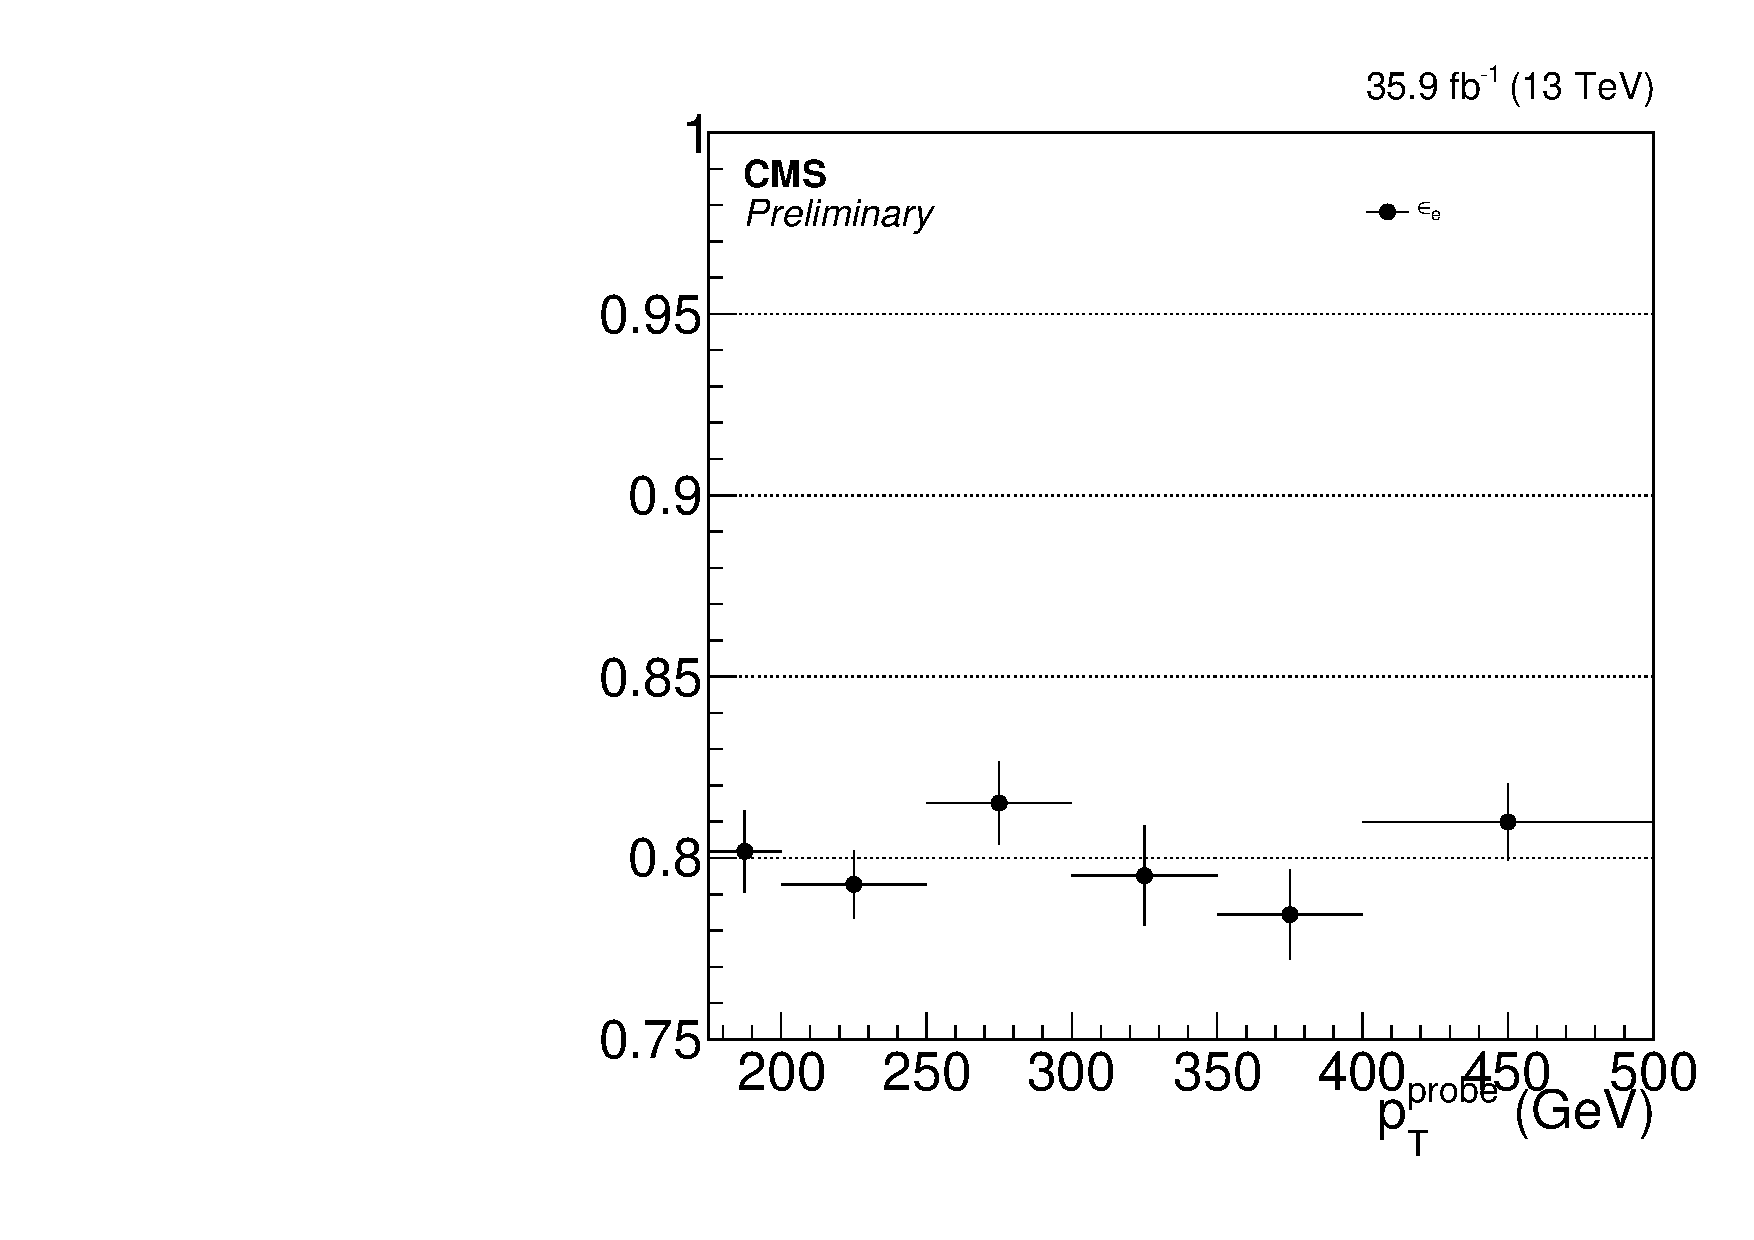
\includegraphics[]{Calibration/Figures/idsf/eff_data_ptalt.pdf}
    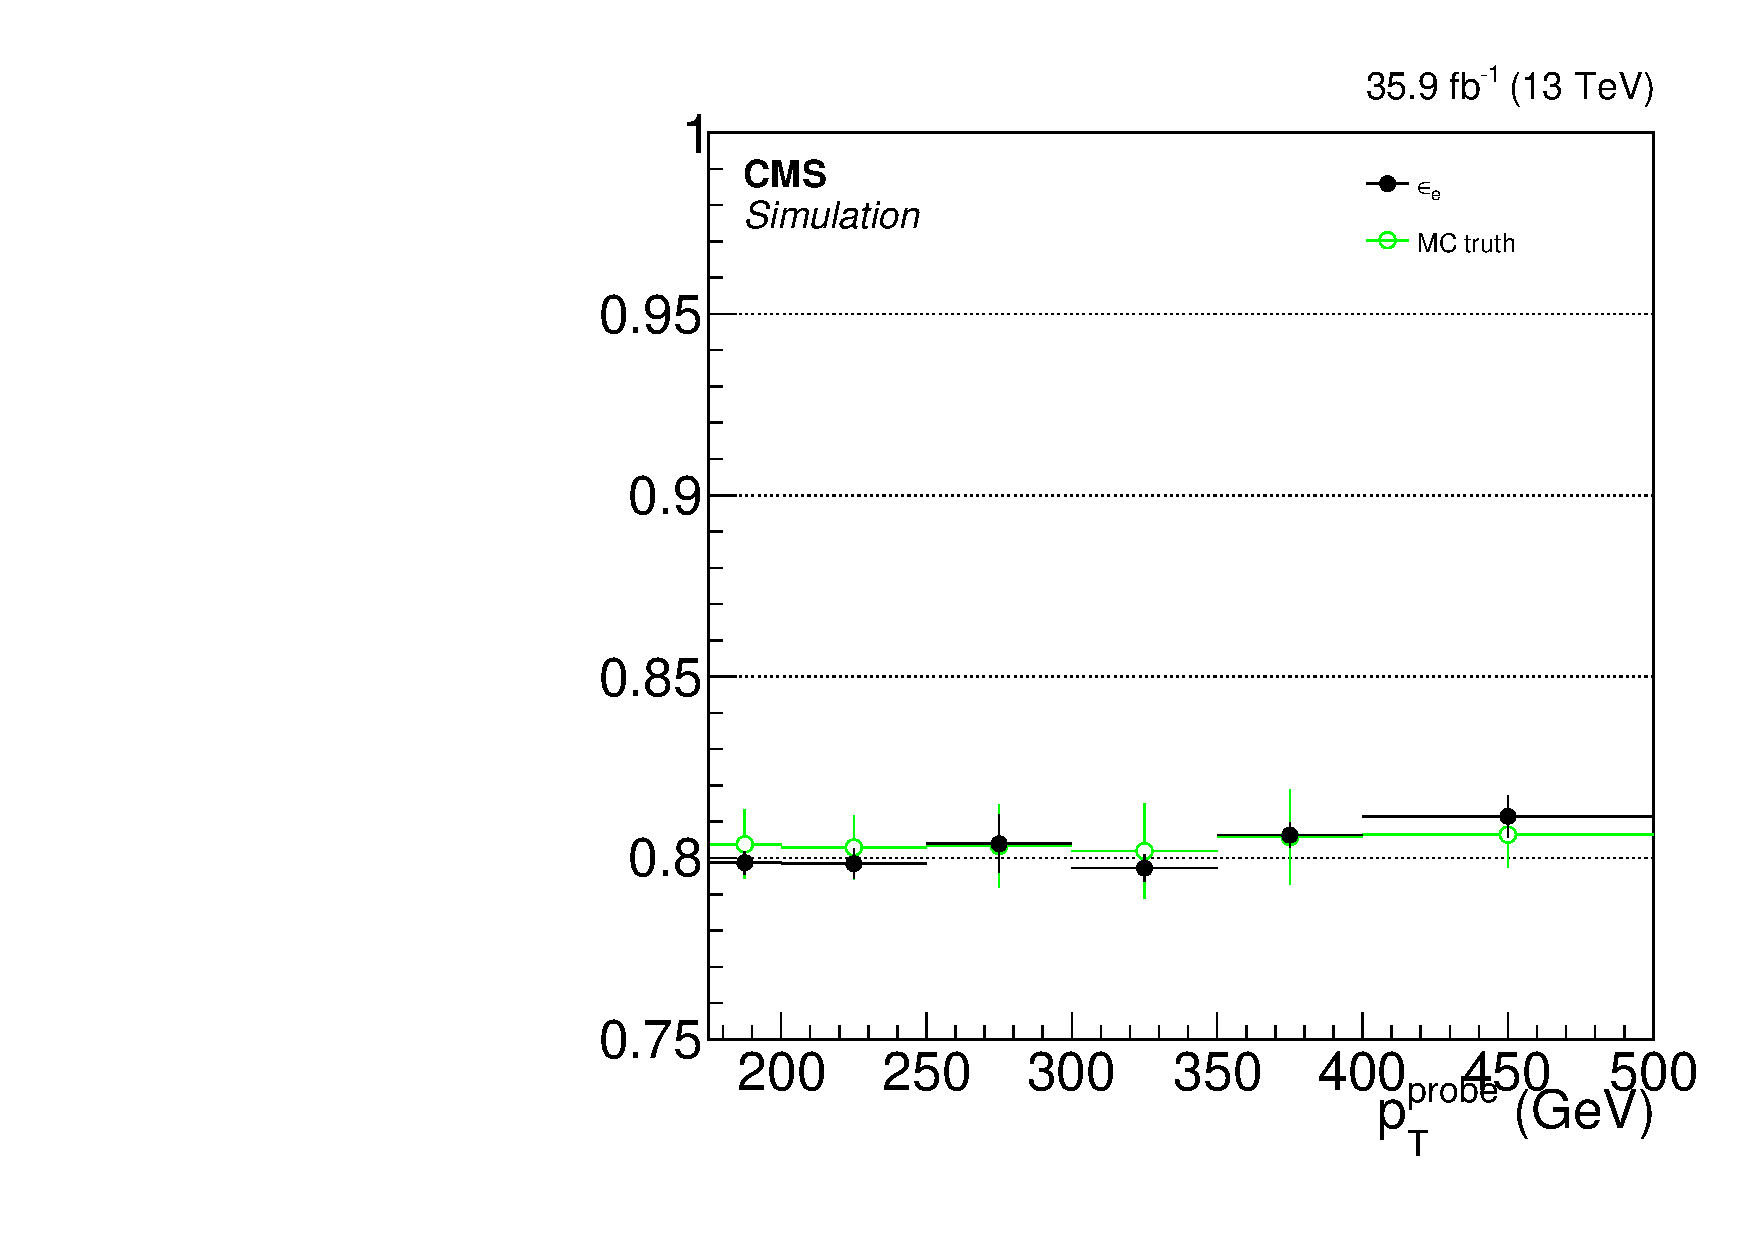
\includegraphics[]{Calibration/Figures/idsf/eff_mc_ptalt.pdf}
  }
  \resizebox{0.5\textwidth}{!}{
    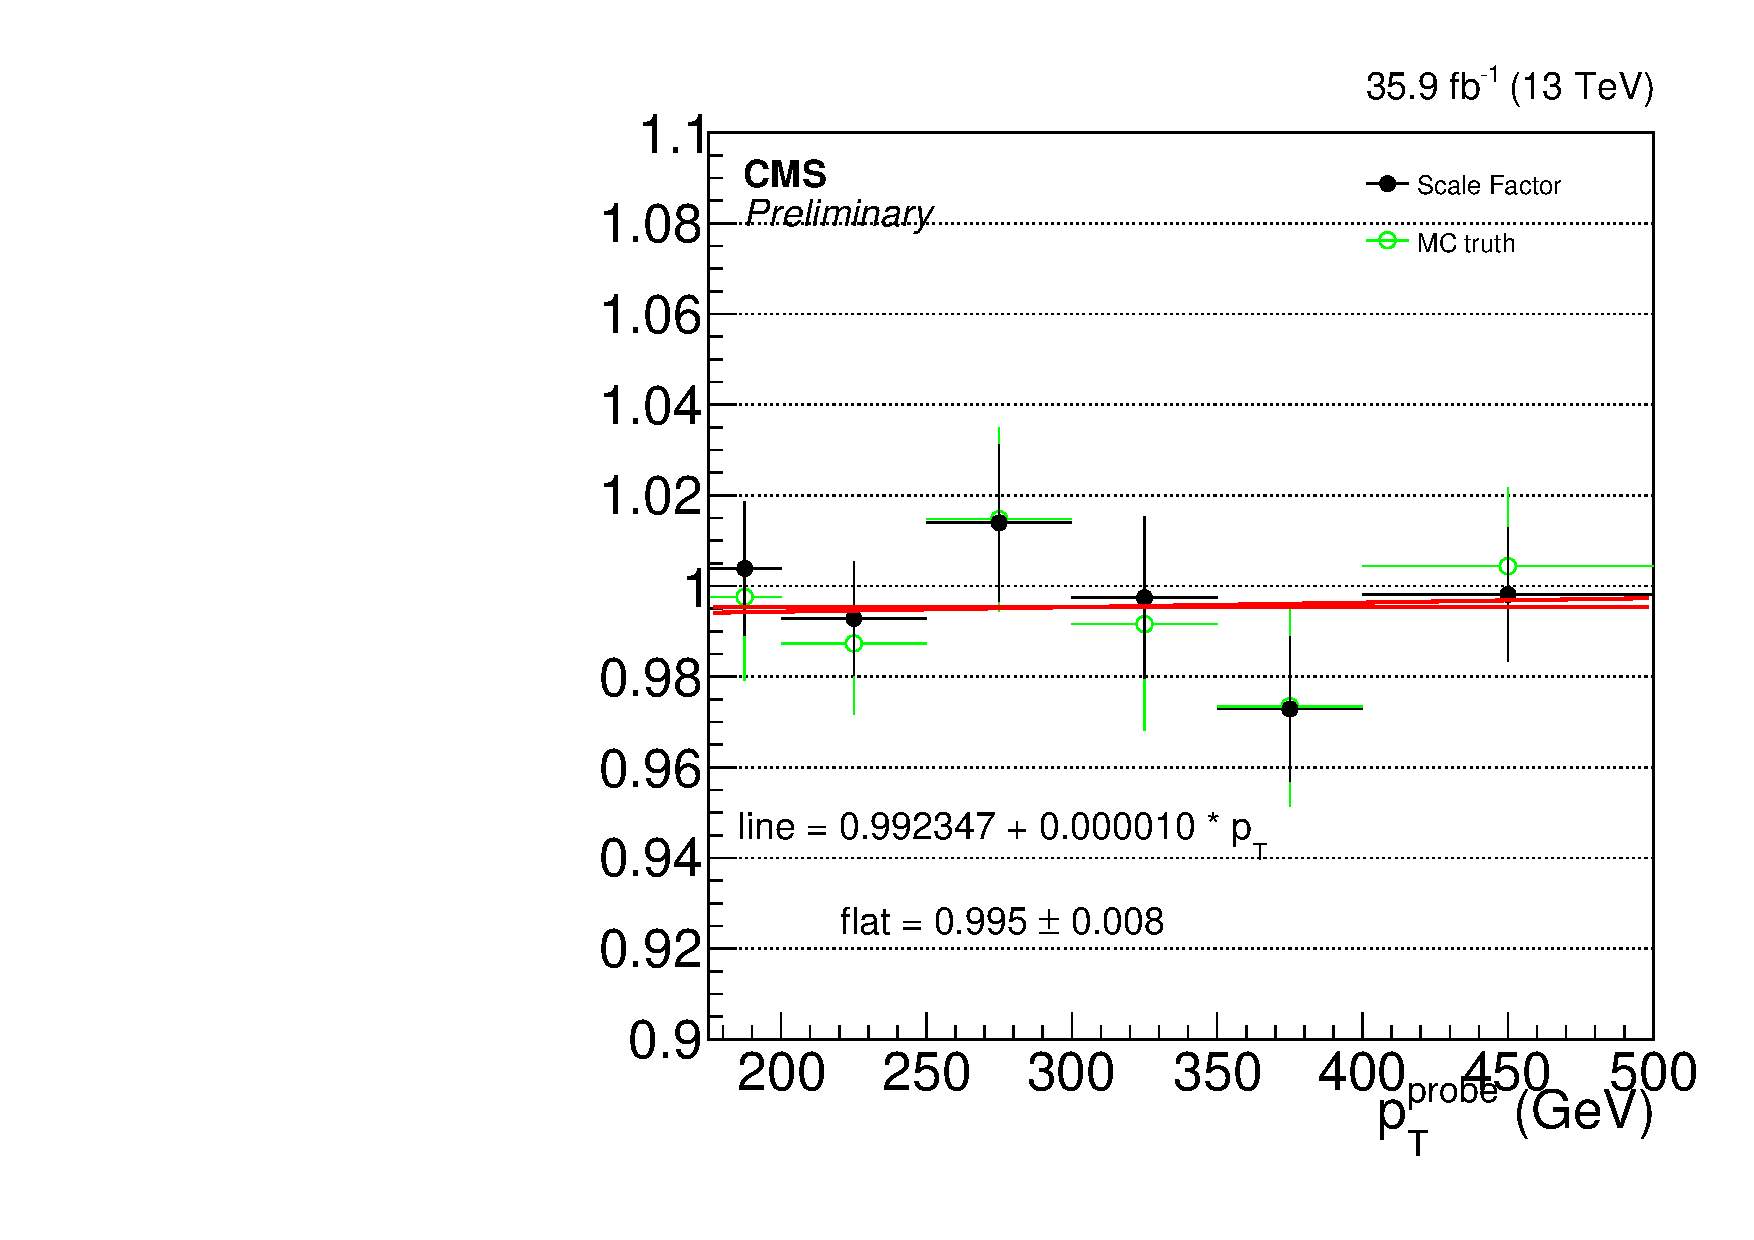
\includegraphics[]{Calibration/Figures/idsf/scaleFactor_ptalt.pdf}
  }
  \caption{
    \egamma\ component of the photon identification efficiency for data (top-left) and MC (top-right) and correspending scale factor (bottom) as a function of photon \pt.
  }
  \label{fig:idsf_results}
\end{figure}

The MC efficiency is taken from counting the number truth-matched electrons passing and failing the \egamma\ part of the ID from a \Zee\ sample. 
Additionally, the MC efficiency is computed using the same procedure as in data as a cross-check.
The efficiencies obtained from these two methods are consistent within their uncertainties. 

\begin{table}[htbp]
  \centering
  \begin{tabular}{ c|c|c }
    $\pt^{\mathrm{probe}}$ (GeV) & MC Fit & Truth \\\hline
    (175, 200)  & $1.014 \pm 0.008$ & $1.009 \pm 0.016$ \\
    (200, 250)  & $1.003 \pm 0.008$ & $0.999 \pm 0.014$ \\
    (250, 300)  & $1.014 \pm 0.010$ & $1.016 \pm 0.019$ \\
    (300, 350)  & $1.002 \pm 0.014$ & $0.997 \pm 0.022$ \\
    (350, 400)  & $0.986 \pm 0.012$ & $0.987 \pm 0.022$ \\
    (400, 6500)  & $0.988 \pm 0.011$ & $0.999 \pm 0.016$ \\
  \end{tabular}
  \caption{\egamma\ scale factors as a function of photon \pt.}
  \label{tab:idsf_results}
\end{table}

The data efficiencies, MC efficiencies, and resulting scale factors as a function of \pt\ are shown in Figure~\ref{fig:idsf_results}. 
The scalefactors are consistent with unity within the uncertainties. 
The numerical values are given in Table~\ref{tab:idsf_results}. 
We use the bin by bin scale factor corresponding to the truth values in the analysis. %% oops might need to fix
